\documentclass[]{article}
\usepackage[brazil]{babel}
\usepackage{graphicx}
\usepackage{mathtools}
\usepackage{float} 
\usepackage{xcolor}


\usepackage{array}
\usepackage{booktabs}



% margenes
\usepackage[a4paper,left=3cm,right=3cm,top=3cm]{geometry}

%opening
\title{}
\author{}

\begin{document}

\begin{center}
	{\tiny {\normalsize {\large Lista de exercicios 3\\
Transferência de calor e mecânica dos fluidos computacional I\\
\textbf{Cristian Herledy Lopez Lara}}}}
\end{center}

\section*{Exercício 3.1}
\subsubsection*{4.1}

No caso das oscilações numéricas, são efeitos que surgem da utilização de sistemas de interpolação espacial linear que geram erros de truncamento (justamente por serem aproximações). No caso de oscilação, os erros associados são erros não dissipativos como os gerados pelo sistema CDS, ou os derivados da utilização de diferenças centrais. Essas oscilações aparecem aproximando valores de propriedades transportadas pelo fluxo com médias espaciais (interpolações) geram perturbações no fluxo distantes da solução real. Esses erros são atenuados com o refinamento da malha, justamente porque a aproximação é melhorada espacialmente e, portanto, o erro de truncamento associado diminui. No caso da difusão numérica, deriva do aparecimento de erros de truncamento de natureza dissipativa associados a termos advectivos. Como a interpolação não é exata, suas aproximações adicionam erros, que também podem ser tratados com o refinamento da malha, mas não eliminados.\\

\subsubsection*{4.2}

A divisão espacial, que é o próprio ato de utilizar uma malha, gera erros de truncamento ao aplicar aproximações com funções de interpolação devido à natureza discreta do uso da técnica. A verdadeira solução vem da ideia do regime contínuo. Numericamente, discretizações temporais e espaciais são usadas para chegar discretamente o mais próximo possível de uma solução completamente contínua para o problema físico. Malhas menores têm efeito direto na redução de erros de truncamento, pois a discretização se aproxima da solução contínua ou real.

\subsubsection*{4.3}

A equação unidimensional para o problema de convecção e difusão em regime permanente é

\begin{equation}
	\frac{\partial}{\partial x} \left( \rho u \phi \right) = \frac{\partial}{\partial x} \left( \Gamma^\phi \frac{\partial \phi}{\partial x} \right)
\end{equation}

Integrando no espaço obtemos\\

\begin{equation}
	 \rho u \phi _e -  \rho u \phi_w =  \varGamma^\phi \frac{\partial \phi}{\partial x}\arrowvert_e - \varGamma^\phi \frac{\partial \phi}{\partial x}\arrowvert_w
\end{equation}


Aproximando os fluxos usando diferenças centrais CDS como interpolação linear, usamos as seguintes expressões

\begin{equation}
	\begin{aligned}
		\phi_{e} = \dfrac{\phi_{E} + \phi_{P}}{2} \\
		\phi_{w} = \dfrac{\phi_{W} + \phi_{P}}{2} \\
	\end{aligned}
\end{equation}

\begin{equation}
	\begin{aligned}
		\frac{\partial\phi}{\partial x}\bigg|_{e} = \frac{\phi_{E}-\phi_{P}}{\Delta x_{e}}\\
		\frac{\partial\phi}{\partial x}\bigg|_{w} = \frac{\phi_{P}-\phi_{W}}{\Delta x_{w}}\\
	\end{aligned}
\end{equation}

Com variações na velocidade, diferentes casos são plotados com aumento no efeito de difusão.


Observam-se oscilações com velocidades maiores, devido à geração de coeficientes negativos por à utilização do CDS como sistema de interpolação espacial. O aumento da velocidade traz efeitos de difusão aumentados, que o CDS não trata adequadamente.\\

Incorporando UDS em termos advectivos

\begin{equation}
	\begin{aligned}
		\phi_e = \phi_p\\
		\phi_w = \phi_W\\
	\end{aligned}	
\end{equation}\\

\begin{figure}[H]
	\centering
	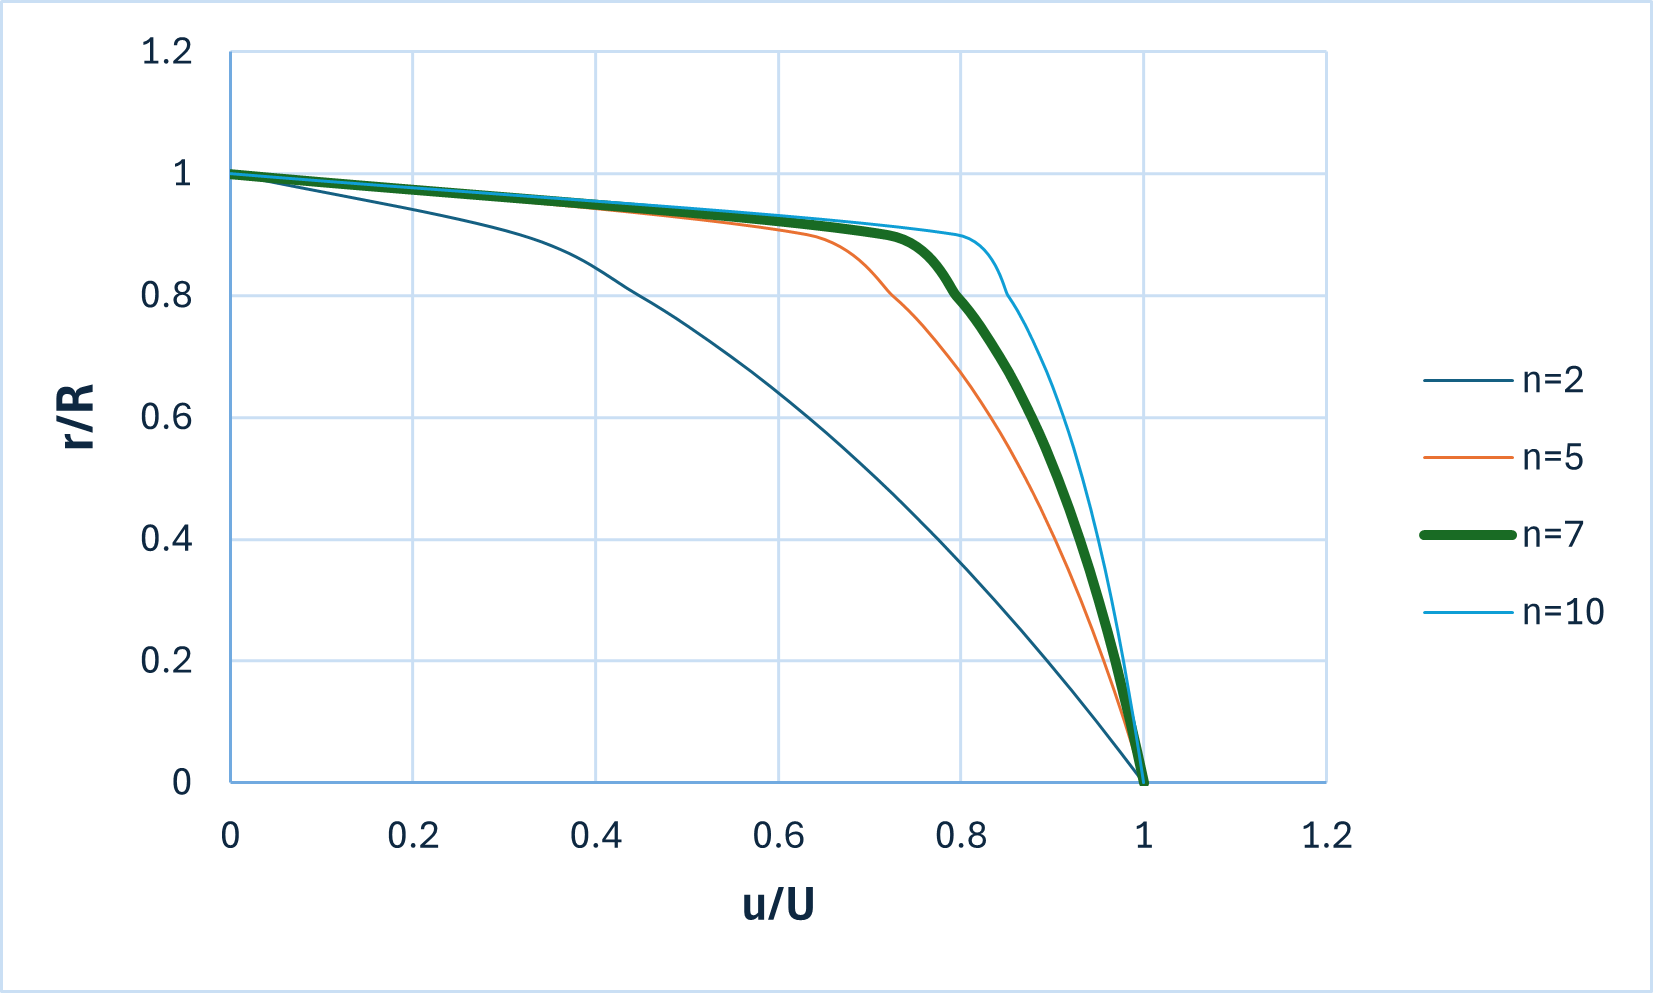
\includegraphics[width=.65\textwidth]{Figures/1.png}
	\caption{Evolução do Phi no espaço UDS}
\end{figure}




\end{document}





